\documentclass[10pt]{article}
\usepackage{tikz}
\usetikzlibrary{shapes.misc}
\usepackage[margin=0cm]{geometry}
\pagestyle{empty}
\tikzstyle{every node}=[cross out, draw, red]

\begin{document}

\vspace*{\fill}
\begin{center}
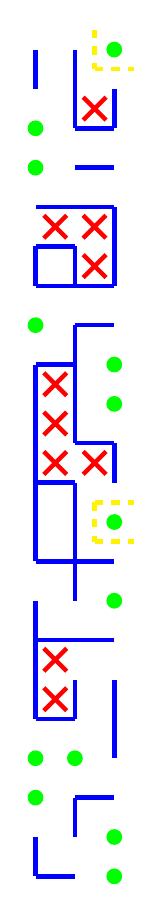
\begin{tikzpicture}[x=0.5cm, y=-0.5cm, ultra thick, blue]
% Walls
    \draw (1,2) -- (2,2);
    \draw (1,3) -- (2,3);
    \draw (0,4) -- (2,4);
    \draw (0,5) -- (1,5);
    \draw (0,6) -- (2,6);
    \draw (1,7) -- (2,7);
    \draw (0,8) -- (1,8);
    \draw (1,10) -- (2,10);
    \draw (0,11) -- (1,11);
    \draw (0,13) -- (2,13);
    \draw (0,15) -- (2,15);
    \draw (0,17) -- (1,17);
    \draw (1,19) -- (2,19);
    \draw (0,21) -- (1,21);
    \draw (0,0) -- (0,1);
    \draw (0,5) -- (0,6);
    \draw (0,8) -- (0,13);
    \draw (0,14) -- (0,17);
    \draw (0,20) -- (0,21);
    \draw (1,0) -- (1,2);
    \draw (1,5) -- (1,6);
    \draw (1,7) -- (1,10);
    \draw (1,11) -- (1,14);
    \draw (1,16) -- (1,17);
    \draw (1,19) -- (1,20);
    \draw (2,1) -- (2,2);
    \draw (2,4) -- (2,6);
    \draw (2,10) -- (2,11);
    \draw (2,16) -- (2,18);
% Pillars
    \fill[green] (2,0) circle(0.2);
    \fill[green] (0,2) circle(0.2);
    \fill[green] (0,3) circle(0.2);
    \fill[green] (0,7) circle(0.2);
    \fill[green] (2,8) circle(0.2);
    \fill[green] (2,9) circle(0.2);
    \fill[green] (2,12) circle(0.2);
    \fill[green] (2,14) circle(0.2);
    \fill[green] (0,18) circle(0.2);
    \fill[green] (1,18) circle(0.2);
    \fill[green] (0,19) circle(0.2);
    \fill[green] (2,20) circle(0.2);
    \fill[green] (2,21) circle(0.2);
% Inner points in accessible cul-de-sacs
    \node at (1.5,1.5) {};
    \node at (0.5,4.5) {};
    \node at (1.5,4.5) {};
    \node at (1.5,5.5) {};
    \node at (0.5,8.5) {};
    \node at (0.5,9.5) {};
    \node at (0.5,10.5) {};
    \node at (1.5,10.5) {};
    \node at (0.5,15.5) {};
    \node at (0.5,16.5) {};
% Entry-exit paths without intersections
    \draw[dashed, yellow] (1.5,0.5) -- (2.5,0.5);
    \draw[dashed, yellow] (1.5,11.5) -- (2.5,11.5);
    \draw[dashed, yellow] (1.5,12.5) -- (2.5,12.5);
    \draw[dashed, yellow] (1.5,-0.5) -- (1.5,0.5);
    \draw[dashed, yellow] (1.5,11.5) -- (1.5,12.5);
\end{tikzpicture}
\end{center}
\vspace*{\fill}

\end{document}
